\chapter{Введение}
 настоящее время исследование процессов происходящих в сердце имеет
приоритетное значение ввиду множества причин. Одной из наиболее важных является
проблема сердечно-сосудистых заболеваний в мировом здравоохранении. Данный вид
заболеваний является широко распространенным и весьма летальным: только в 2019
году причинами около 17.9 миллионов смертей, что составляет примерно 32\% всех
смертей в мире, являлись сердечно-сосудистые заболевания \cite{who}. Таким
образом, в рамках исследования возникает потребность в большом количестве
экспериментов для анализа частотных и пространственно-временных параметров
биоэлектрической активности сердца.

На сегодняшний день одним из самых эффективных методов изучения
биоэлектрических свойств миокарда является метод записи электрограмм с
микроэлектродных матриц. В отличие от классической электрокардиографии (ЭКГ),
которая фиксирует электрические потенциалы на поверхности тела, электрограммы
обеспечивают запись сигналов непосредственно с внутренней поверхности сердца,
что предоставляет более точную информацию о его функционировании. Однако же
вместе с преимуществом данного метода у исследователя возникает ряд проблем:

\begin{enumerate}
	\item Объем данных: Обработка большого объема электрограмм требует
	значительных вычислительных ресурсов и времени, особенно если анализ
	проводится вручную или при использовании традиционных методов. Более того,
	ручной анализ подвержен ошибкам.

	\item Шумы и артефакты: Электрограммы могут содержать различные шумы и
	артефакты, такие как электрические помехи, технические ошибки, которые
	могут искажать данные и затруднять их интерпретацию.

	\item Разнообразие данных: Электрограммы могут различаться по качеству,
	разрешению, формату записи и другим характеристикам. Так же особая
	сложность представляется в нестабильности формы, амплитуды и частоты
	регистрируемых биоэлектрических потенциалов в зависимости от условий
	эксперимента. Все это усложняет исследование и анализ.
\end{enumerate}

Решение вышеописанных проблем требует разработки инновационных методов обработки данных,
автоматизации процессов анализа и разработки специализированных инструментов и
алгоритмов для работы с электрограммами.

Данная работа представляет в качестве решения метод применения машинного, а в
частности глубокого, обучения, представляющий из себя мощное решение для
автоматизации анализа большого количества электрограмм. Для детекции участков
активации предлагается использовать одномерный вариант сверточной нейронной
сети UNet, хорошо себя зарекомендовавшей в задачах сегментации сигнала \cite{victor}.

\section{Обзор литературы}
Обычно сегментация сигнала состоит из двух шагов \cite{ecg-segmentation}:

\begin{enumerate}
	\item Предобработка сигнала --- преобразование или фильтрация для того,
	чтобы выделить интересующую область. В качестве инструментов для этой цели
	могут быть использованы: преобразование Фурье, разнообразные фильтры.

	\item Непосредственно нахождение точек интереса.

\end{enumerate}

Для второго шага могут быть использованы как прямые методы, основанные на
каких-либо эвристиках \cite{euristic-1, euristic-2, euristic-3, euristic-4,
	euristic-5} или же универсальные аппроксиматоры --- нейронные сети
\cite{victor}.

Рассмотрим эти методы более детально. Начнем с прямых:

\vspace*{\baselineskip}

\noindent
\begin{minipage}[t]{.45\textwidth}
	\begin{center}
		\textbf{Преимущества}
	\end{center}

	\begin{enumerate}
		\item Простота реализации: Прямые методы сегментации могут быть
		относительно просты в реализации и понимании, что делает их доступными
		для исследователей и специалистов без глубоких знаний в области
		машинного обучения.

		\item Высокая скорость работы: В некоторых случаях прямые методы могут
		обеспечить более высокую скорость обработки данных.
	\end{enumerate}
\end{minipage}
\hfill
\begin{minipage}[t]{.45\textwidth}
	\begin{center}
		\textbf{Недостатки}
	\end{center}

	\begin{enumerate}
		\item Требуют хорошо настроенных параметров: Для достижения хороших
		результатов прямые методы сегментации требуют тщательной настройки
		параметров, что может быть трудоемким и не всегда интуитивным.

		\item Чувствительность к шуму и вариациям данных: Прямые методы могут
		быть менее устойчивы к шуму и изменчивости данных, что может привести к
		менее точным результатам при анализе сложных или зашумленных сигналов.
	\end{enumerate}
\end{minipage}

\vspace*{\baselineskip}

Для непрямых методов справедливо следующее:

\vspace*{\baselineskip}

\noindent
\begin{minipage}[t]{.45\textwidth}
	\begin{center}
		\textbf{Преимущества}
	\end{center}

	\begin{enumerate}
		\item Автоматическое изучение признаков: Глубокие нейронные сети
		способны автоматически извлекать признаки из данных, что позволяет им
		адаптироваться к разнообразным условиям.

		\item Высокая точность: В результате обучения на больших объемах данных
		глубокие нейронные сети могут достигать высокой точности в сегментации.

		\item Обобщение: Глубокие нейронные сети могут обобщать обученные
		знания на новые данные, что делает их более универсальными и
		применимыми для различных типов сигналов.
	\end{enumerate}
\end{minipage}
\hfill
\begin{minipage}[t]{.45\textwidth}
	\begin{center}
		\textbf{Недостатки}
	\end{center}

	\begin{enumerate}
		\item Требовательность к данным и вычислительным ресурсам: Обучение
		глубоких нейронных сетей требует больших объемов данных и
		вычислительной мощности, что может быть ограничивающим фактором для
		некоторых приложений.

		\item Необходимость оптимизации и настройки: Для достижения оптимальной
		производительности глубокие нейронные сети требуют тщательной
		оптимизации и настройки гиперпараметров, что может потребовать
		значительного времени и усилий.
	\end{enumerate}
\end{minipage}


\newpage
В данной работе была использована комбинация прямых и нейросетевых методов для
достижения лучших результатов. Нейросетевой подход применялся для локализации
местоположения точки интереса в сигналах, в то время как прямые методы
использовались для точного обнаружения этой точки. Такая комбинация позволила
достичь более высокой точности и эффективности в обнаружении интересующих
объектов в исследуемых данных.

\section{Постановка задачи}

Требуется разработать программное обеспечение для анализа многоканальных
электрограмм (для примера см. рис. \ref{fig:egms}). Электрограммы
предварительно размечены экспертом и представляют собой данные о электрической
активности сердца крысы. Задача заключается в создании алгоритма, способного с
большой точностью распознавать и отмечать точки активации для последующего
анализа предметным специалистом.

\begin{figure}[!htb]
	\centering
	\caption{Пример электрограммы (несколько каналов)}
	\label{fig:egms}
	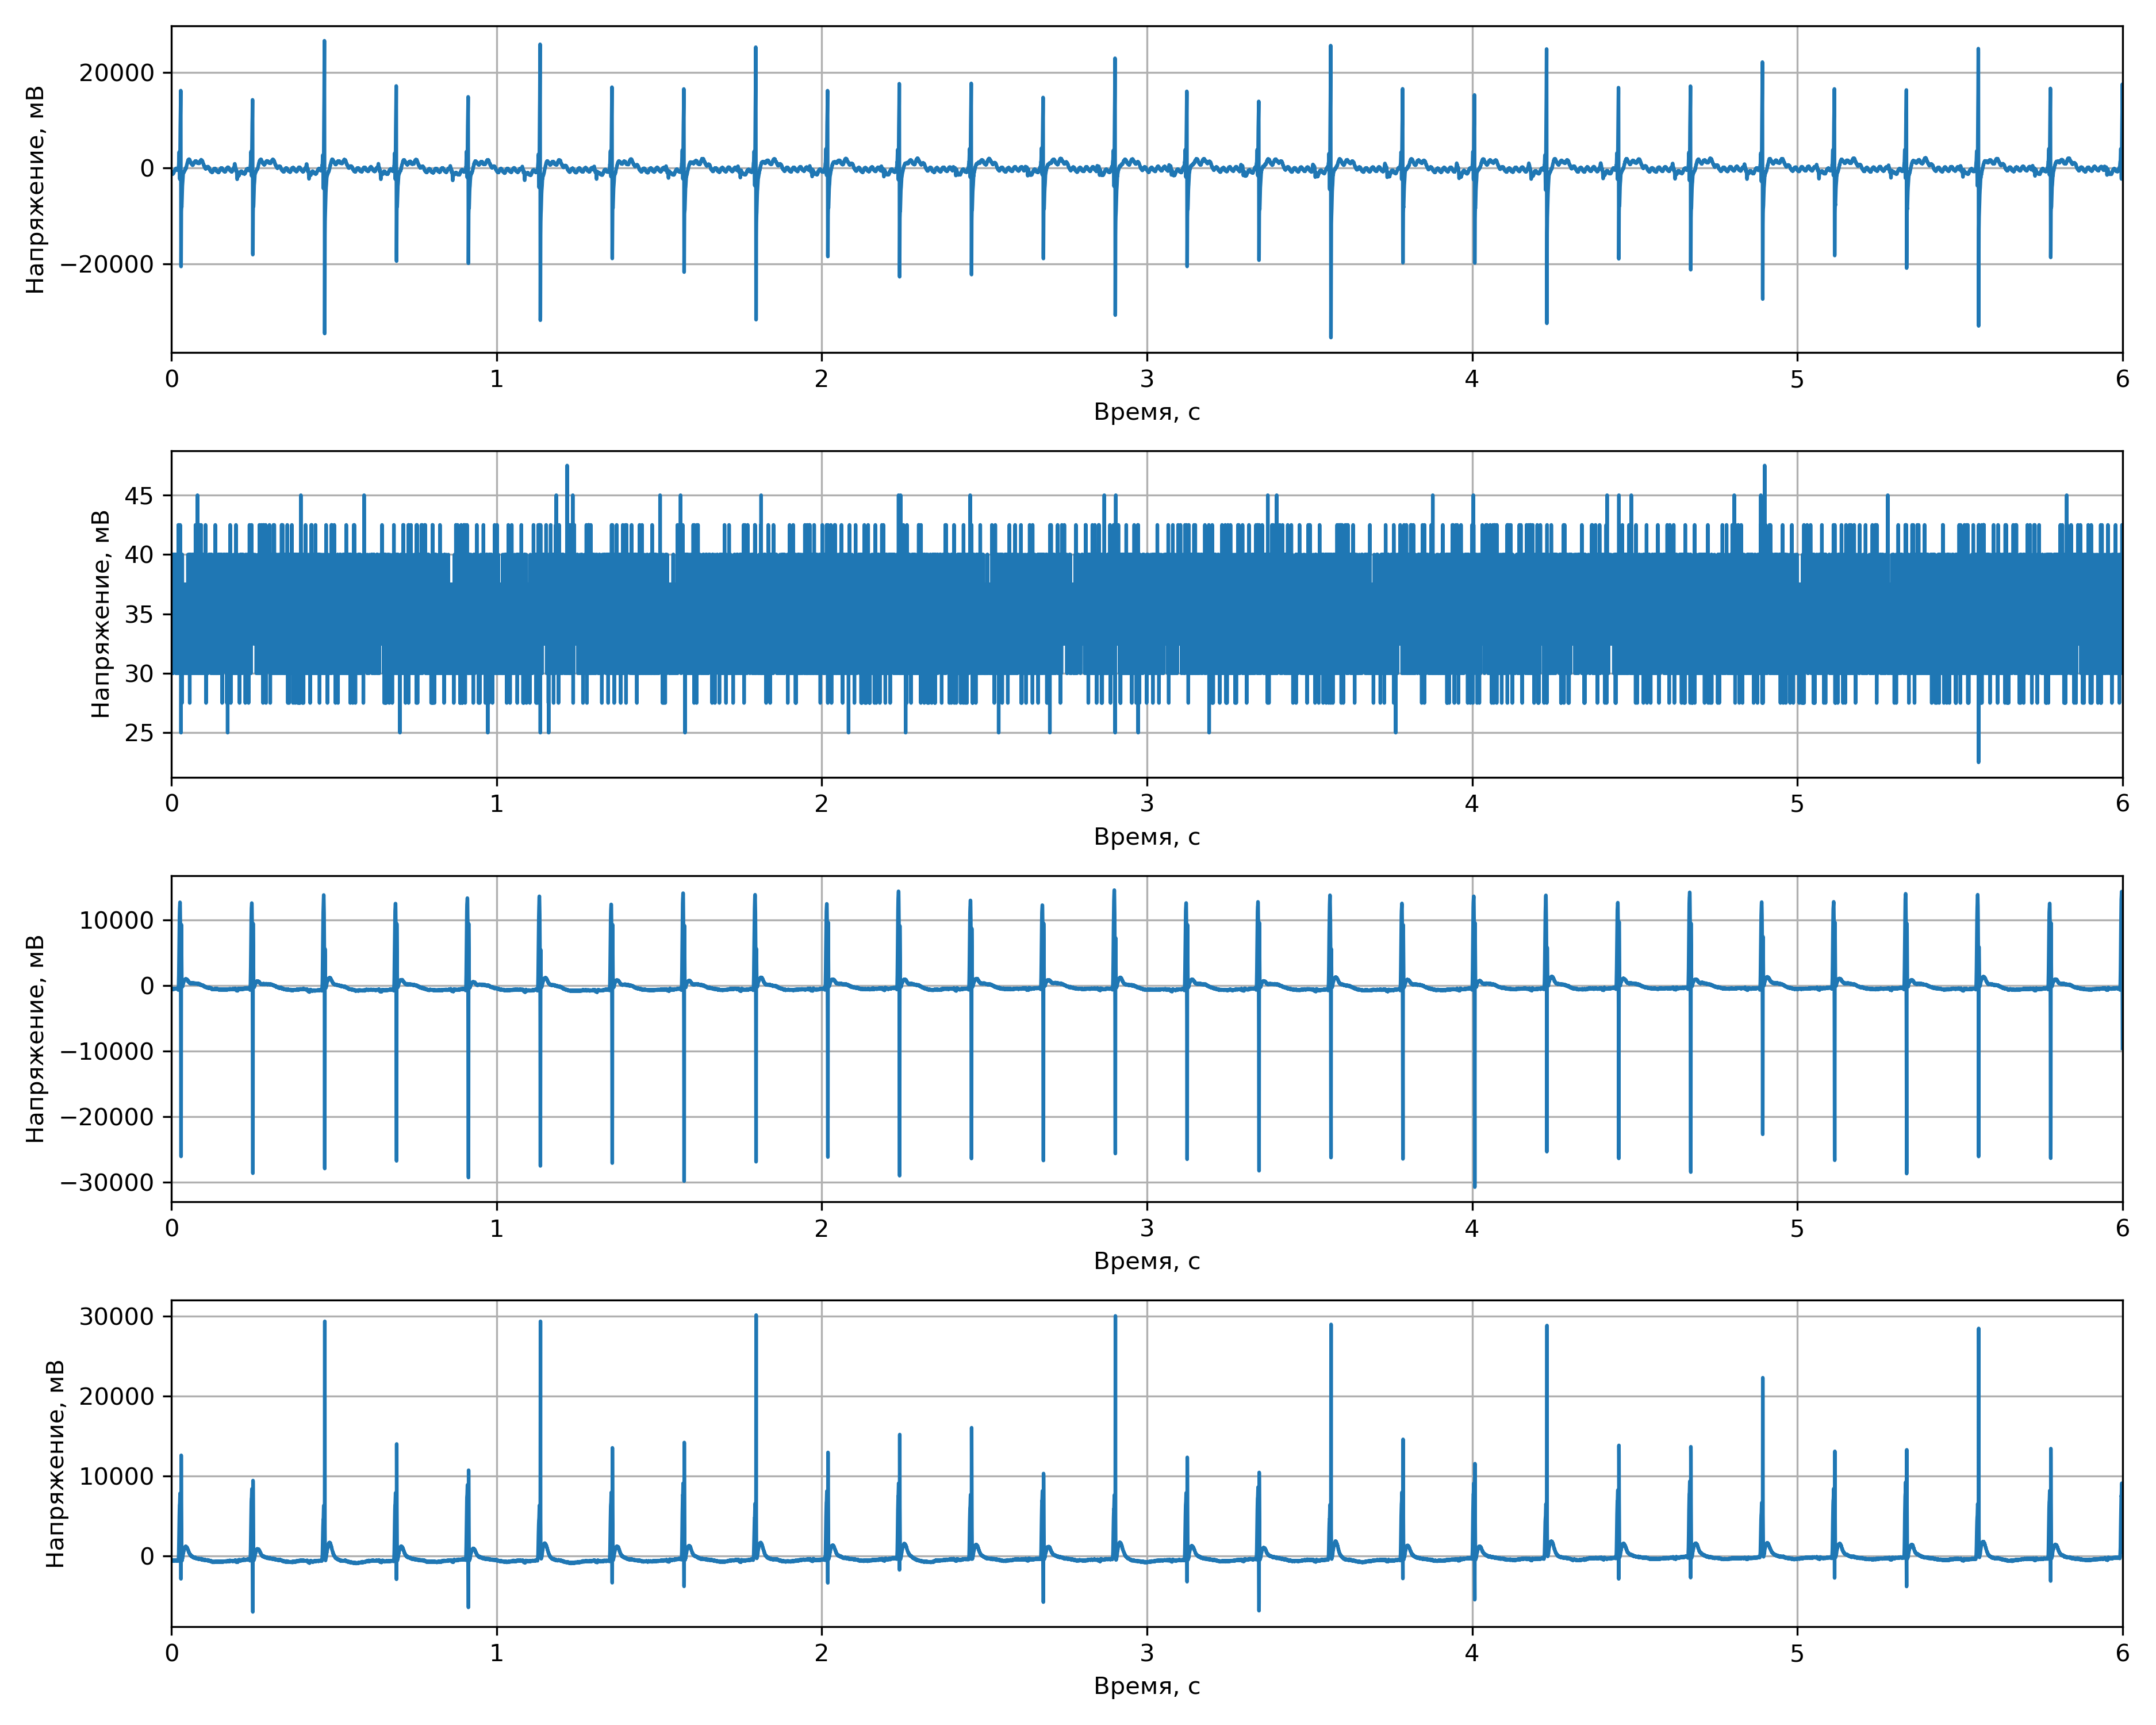
\includegraphics[width=\textwidth]{egms}
\end{figure}
